\documentclass[12pt]{article}
\usepackage{fancyhdr} 
\pagestyle{fancy}
\fancyhf{}
\rhead{Implementación de internet de las cosas}
\rfoot{\thepage}

\usepackage{chngcntr}
\counterwithin{figure}{section}

\usepackage{hyperref}
\hypersetup{
    colorlinks=true,
    linkcolor=blue,
    filecolor=magenta,      
    urlcolor=cyan,
}

\usepackage{graphicx}
\usepackage[spanish, mexico]{babel}
\usepackage{amsmath}
\usepackage{amsthm}
\usepackage{IEEEtrantools}
\usepackage{pgfplots}

% Sections formatting
\usepackage{titlesec}
\titleformat{\section}[hang]
{\Large\normalfont\bfseries}
{\thesection. }{0pt}{}{}

\titleformat{\subsection}[hang]
{\large\normalfont\bfseries}
{}{0pt}{}{}

%%%%%%%%%%%%%%%%%%%%%%%%%%%%%%%%%%%%%%%%%%%%%%%%%%%%%%%%%%%%
\begin{document}
\pagenumbering{roman}
\title{\LARGE{Instituto Tecnológico y de Estudios Superiores
de Monterrey}\\
	\large{Implementación de internet de las cosas (TC1004B): Reto}\\
	\Large{Tarea 5.1: Administración del Reto}\\
	\, \\
	\large{Asesor\\
	Claudia M. Solís Garza}}
\author{
A00827095 -- Omar Enrique González Uresti\\
A00827638 -- Emiliano García Aguirre\\
A00828073 -- Axel Giovanni Villanueva Cuéllar\\
A00828368 -- Jesús Urquidez Calvo\\
A01720388 -- Guillermo Andrés Castillo Chapa
}
\date{\today}
\maketitle
\abstract{Se presenta lo ocurrido mientras se realizó el
pre-inicio, el desarrollo de inicio, y se muestran las
evidencias de la planeación que se tiene para el proyecto.}

\begin{figure}[!t]
\centering

\includegraphics[width = \textwidth]{logo}
\end{figure}

\newpage

\tableofcontents
\newpage

\pagenumbering{arabic}

\section{Pre-Inicio}
Las evidencias de lo que se menciona a continuación se
pueden encontrar en Apéndice \ref{evidencias_PreInicio}.

\subsection{Omar Enrique González Uresti}
Creo que la complejidad de poder realizar la conexión se
debe a la cantidad de cosas técnicas que se deben hacer
previamente. Además, de que tuve errores al conectar el
puerto, sin embargo, supe arreglarlo y pude solucionarlo.

\subsection{Emiliano García Aguirre}
Al realizar la conexión del MCU con mi computadora me topé
con un par de problemas. El primero fue que no había
conectado bien el cable a mi computadora y no registraba el
puerto. Después, cuando intenté conectar el microprocesador
al internet escribí mal mi contraseña varias veces hasta que
finalmente corrió el código como debía. 

\subsection{Axel Giovanni Villanueva Cuéllar}
Con la experiencia previa que tenía programando en Arduino,
efectuar la mayorías de las cosas requeridas lo consideré
como algo muy sencillo de hacer. Como única complicación que
tuve fue la de encontrar un cable que en verdad pasara
información y no fuera sólo de energía, pero a parte de eso
todo corrió sin problemas. Además tras leer el código e
intentar obtener el API para la página usada, se reparó que
lograr lo último no iba a ser posible, y que con lo que se
imprimió en el Panel de Control era suficiente para probar
que había funcionado.

\subsection{Jesús Urquidez Calvo}
No tuve complicación a la hora de aplicar el programa del
LED. Sin embargo a la hora de activar el código de Wifi se
me complicó a la hora de notar el
\verb|Serial.begin(115200)| que estaba diferente y además de
que no se podía conectar a la API ya que el registro en la
página no era posible.

\subsection{Guillermo Andrés Castillo Chapa}
En mi caso yo aprendí que el NodeMCU no accepta redes 5G y
me tardé un poco en enteder el problema, para resolverlo lo
que hice fue agarrar la red 2.4 de mi casa y ya con eso
funcionó bien. Yo nunca había usado Arduino entonces fue un
poco complicado pero ya entendí cómo hacer lo básico.

\section{Inicio}
\subsection{Nombre}
IoP: Internet of Plants\footnote{Un guiño muy directo a la
materia que se está cursando.}.

\subsection{Área a la que pertenece su aplicación}
Medio ambiente, sustentabilidad.

\subsection{Descripción de la aplicación}
Se tiene la intención de diseñar una aplicación que se
encargue de cuidar plantas domésticas\footnote{Si bien se
puede escalar a sistemas más grandes de manera un tanto
sencilla, como ``minimum valuable product'' se hará con solo
una planta en el hogar.}.

El sistema funcionará mediante un sensor de humedad el cual
estará conectado a la planta, y estará brindando la
información de las condiciones de la tierra; con este dato,
se encenderá un LED RGB para ir indicando el estado por
medio de su color, y dependiendo del caso, el sistema
accionará un sistema de riego para la planta.

Asimismo se planea agregar un sensor ultrasónico para
medir la cantidad de agua en el recipiente\footnote{A partir
de la distancia que existe entre el sensor y el agua es como
se espera obtener el resultado. Se resalta que dependiendo
de la capacidad de un sensor ultrasónico de detectar el agua
será lo que decida si esta parte del proyecto se
implementará.}, y de igual manera se contará con un LED RGB
para indicar el nivel de agua.

\subsection{Diagrama}
Se presenta el diagrama con los componentes básicos y el
cómo estarán relacionados entre ellos.

\begin{figure}[!h]
\centering
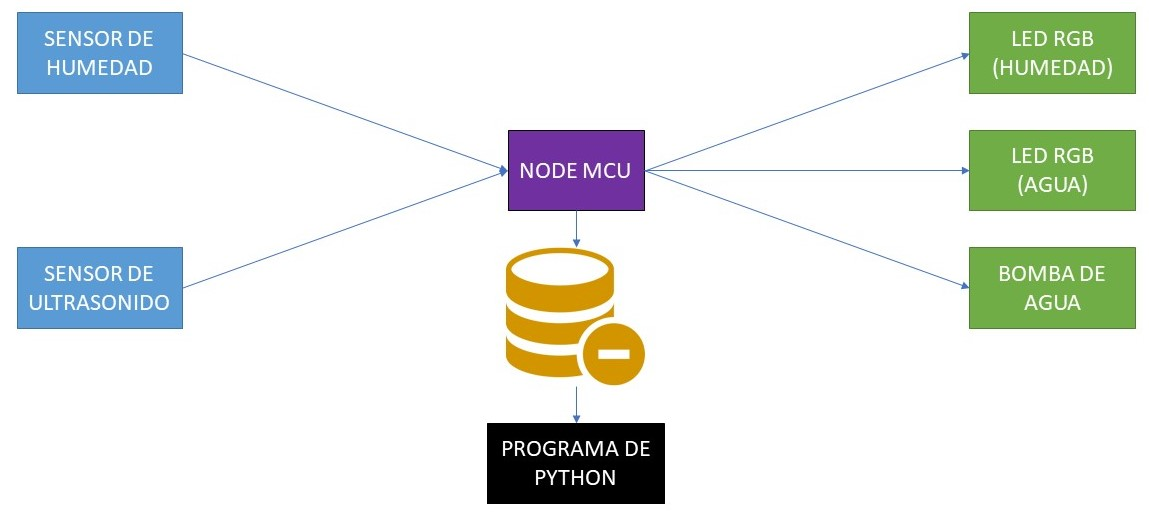
\includegraphics[width = \textwidth]{diagrama}
\end{figure}

\subsection{Lista de los sensores/actuadores}
\begin{itemize}
\item Sensor de humedad.
\item 2 LED RGB.
\item Bomba de agua de 3V.
\item Sensor ultrasónico.
\item Node MCU.
\end{itemize}

\subsection{Visualización de datos}
Se plantea hacer una aplicación para la computadora
elaborada en Python en donde se presenten los datos
obtenidos. De manera preliminar se anticipa usar PyQT en
combinación con Pandas para lograr lo anterior.

La manera de representar la información será mediante
gráficas de tiempo para ilustrar el cambio que ha tenido
conforme pasan los días, así como otras conclusiones que se
puedan plantear a partir de la información recopilada 
(cantidad de agua usada, periodicidad en que se riega la
planta) como datos disponibles para el usuario y así pueda
estar informado de lo más relevante relacionado a su planta.

\section{Planeación}
Para facilitar la colaboración entre los miembros del
equipo se empleará GitHub y se usará
\href{https://github.com/axelgio01/TC1004B.8}{este
repositorio} en donde todos los integrantes ya se
encuentran como colaboradores.

Para la parte de administración de proyecto se usarán las
mismas herramientas que ofrece la plataforma, por lo que
en la sección de
``\href{https://github.com/axelgio01/TC1004B.8/projects/1}{
Projects}'' se encuentran el estado (por hacer, en proceso,
terminado) de las diversas actividades que se tienen
previstas por hacer.

Se destaca de igual manera que en
``\href{https://github.com/axelgio01/TC1004B.8/milestones}{
Milestones}'' se encuentran las fechas importantes que
se tienen previstas\footnote{Son las fechas de entrega
oficial por parte de la clase, pero se agregarán más en caso
de sentir que se requiere realizar un mejor seguimiento},
mientras que en
``\href{https://github.com/axelgio01/TC1004B.8/issues}{
Issues}'' están las actividades que permiten cumplir de
manera satisfactoria las anteriores.

La manera en como está el repositorio actualmente se
encuentra en el Apéndice \ref{evidencia_Planeacion}.

\newpage
\appendix
\section{Evidencias Pre-Inicio}\label{evidencias_PreInicio}
\subsection{Omar Enrique González Uresti}
\begin{figure}[!h]
\centering
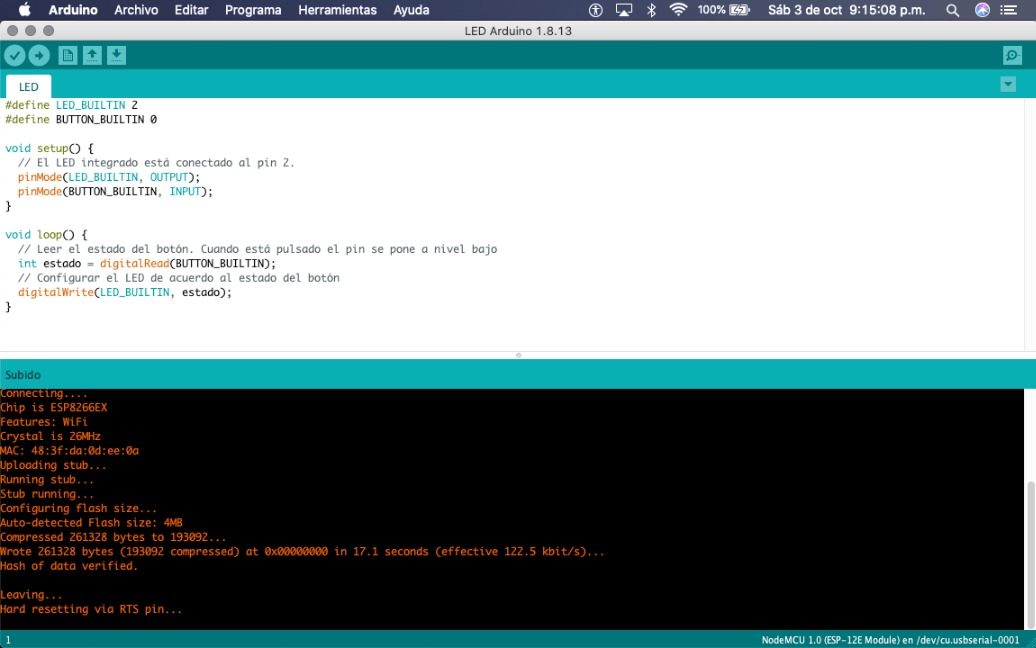
\includegraphics[width = 0.9\textwidth]{omar1}
\end{figure}

\begin{figure}[!h]
\centering
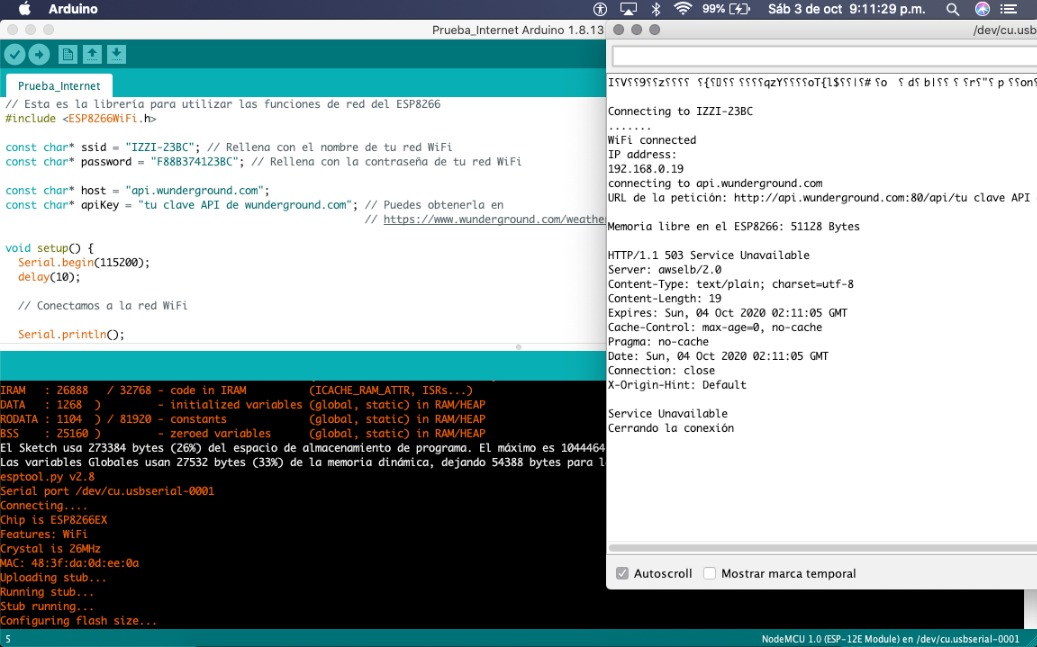
\includegraphics[width = 0.9\textwidth]{omar2}
\end{figure}

\newpage

\subsection{Emiliano García Aguirre}
\begin{figure}[!h]
\centering
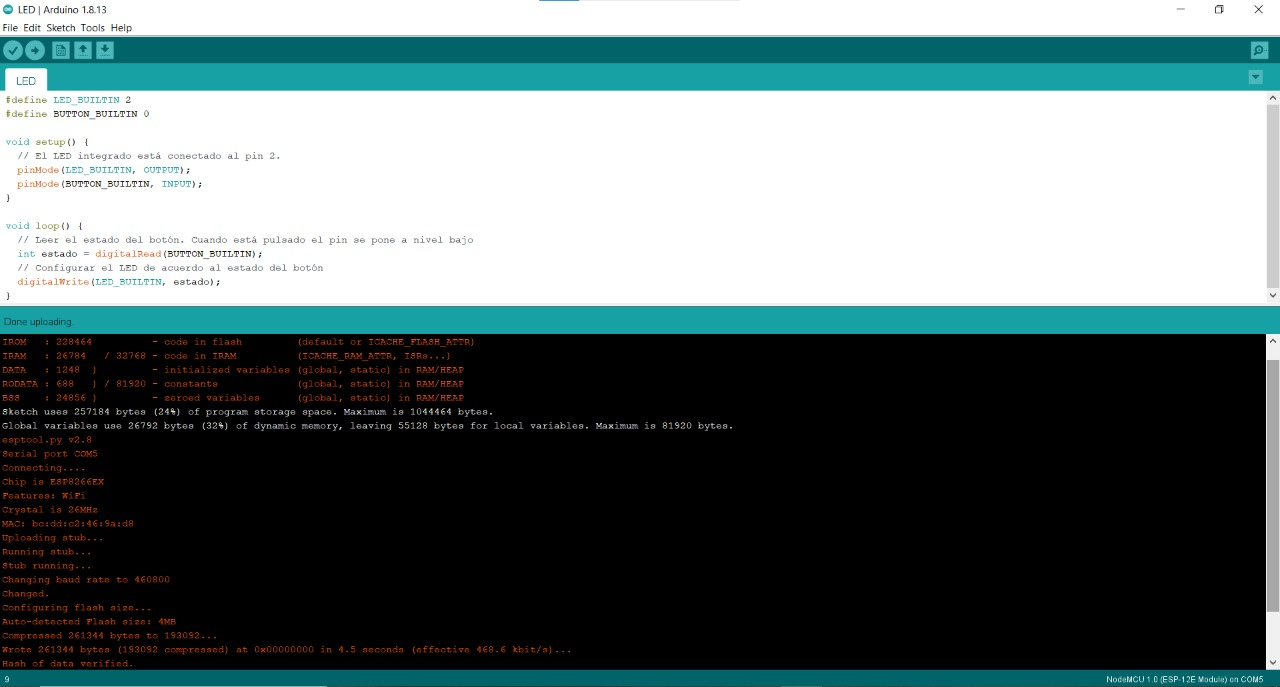
\includegraphics[width = \textwidth]{emi1}
\end{figure}

\begin{figure}[!h]
\centering
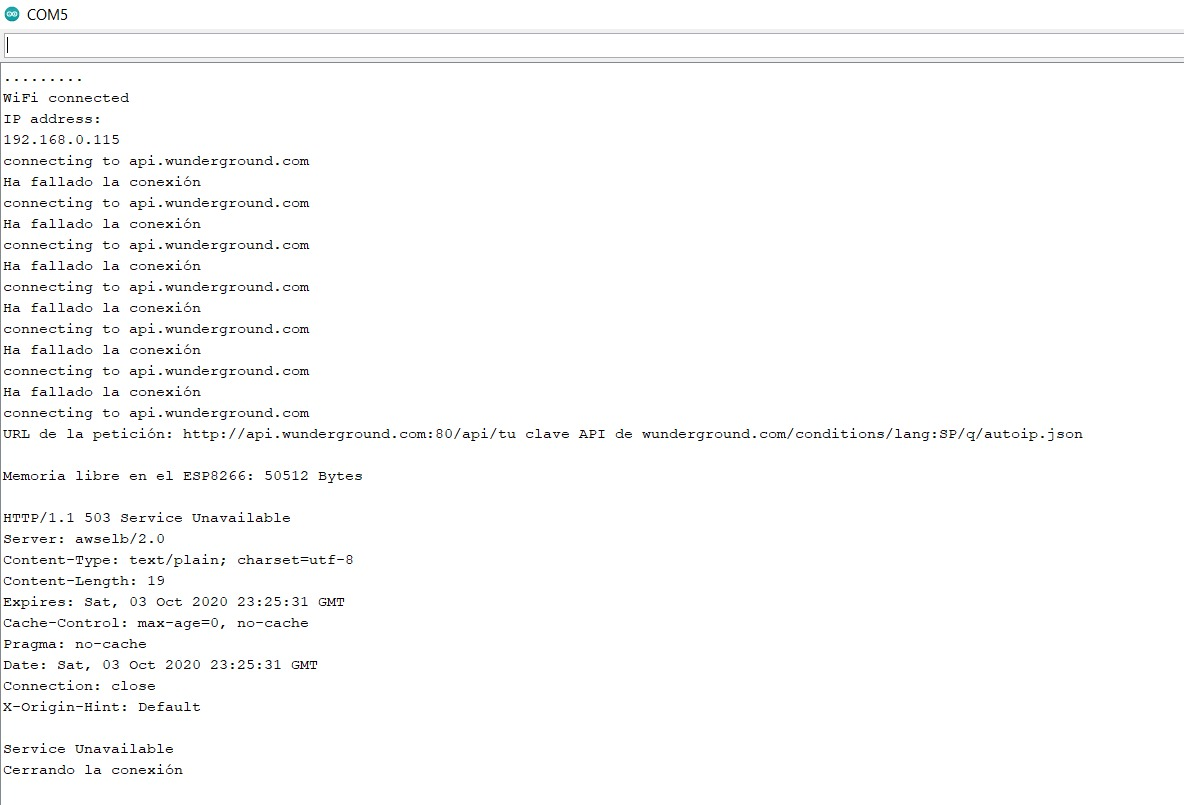
\includegraphics[width = \textwidth]{emi2}
\end{figure}

\newpage

\subsection{Axel Giovanni Villanueva Cuéllar}
\begin{figure}[!h]
\centering
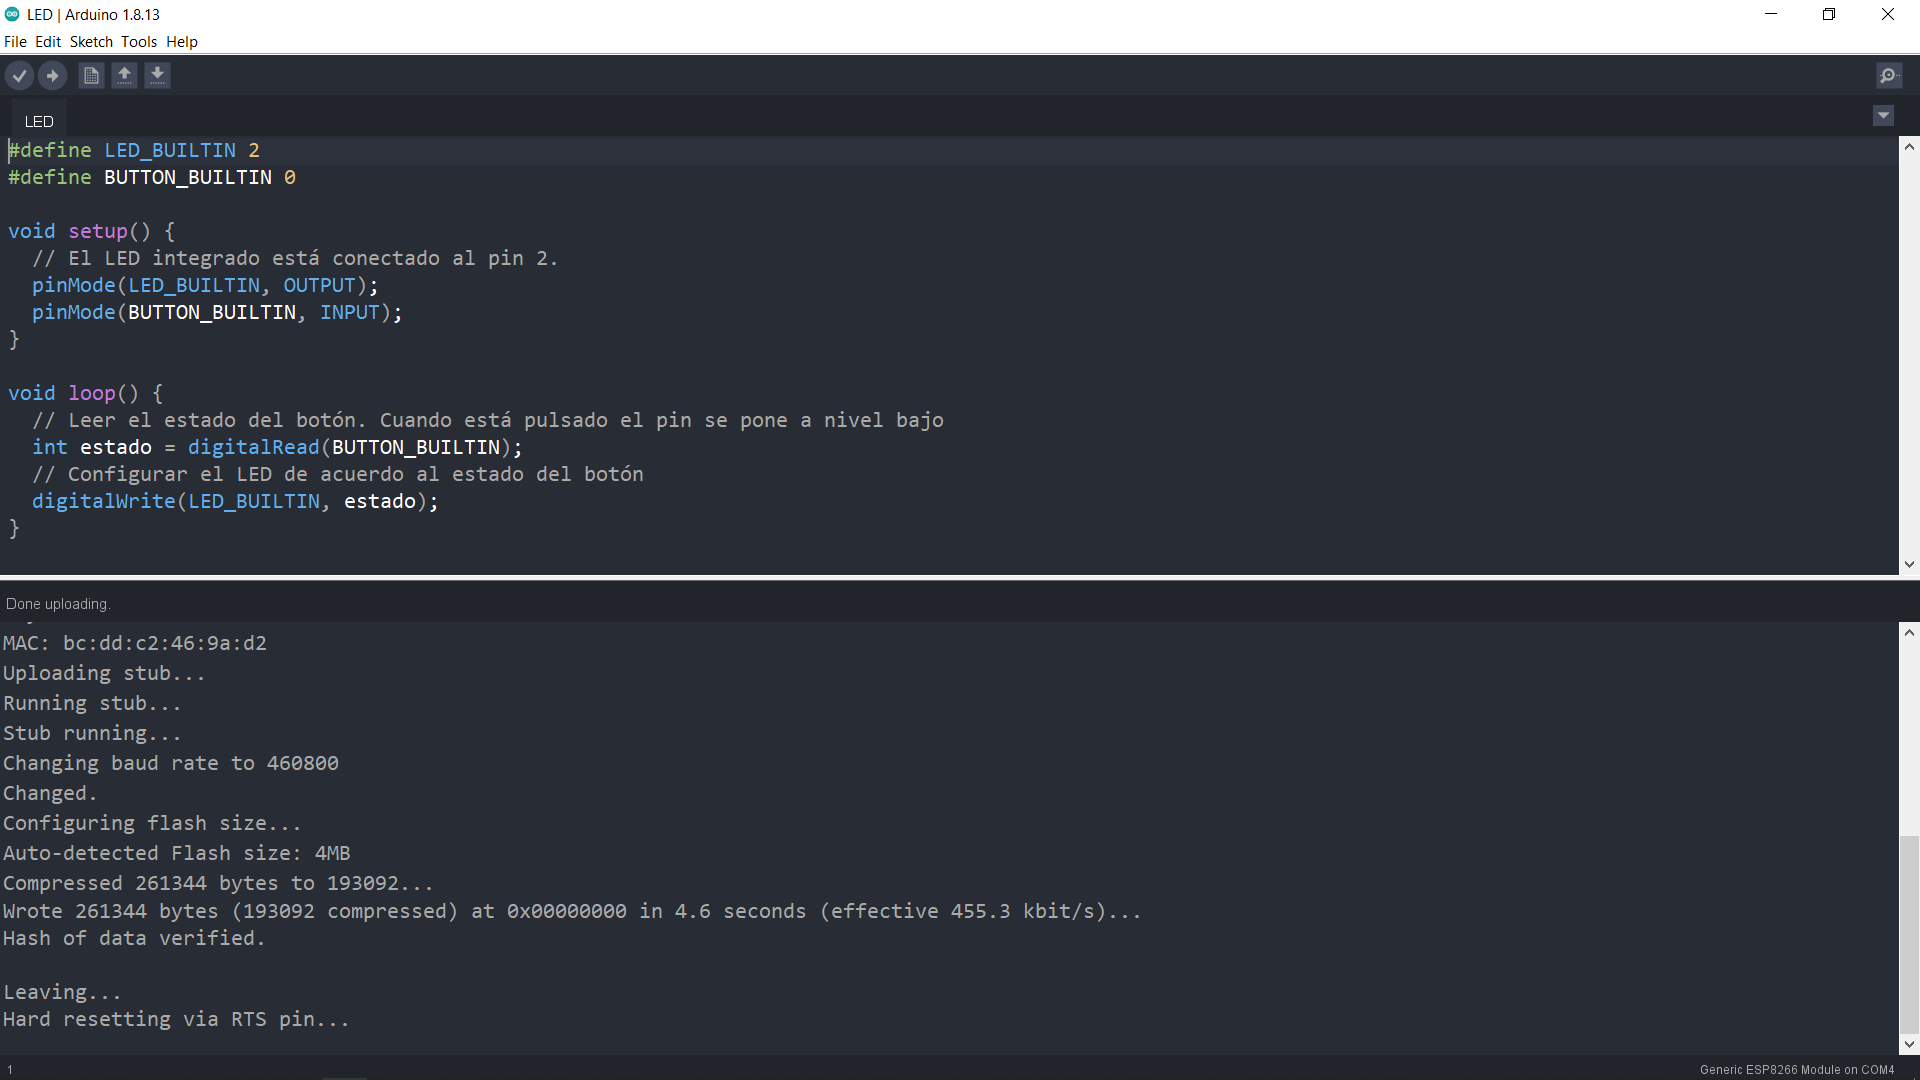
\includegraphics[width = \textwidth]{axel1}
\end{figure}

\begin{figure}[!h]
\centering
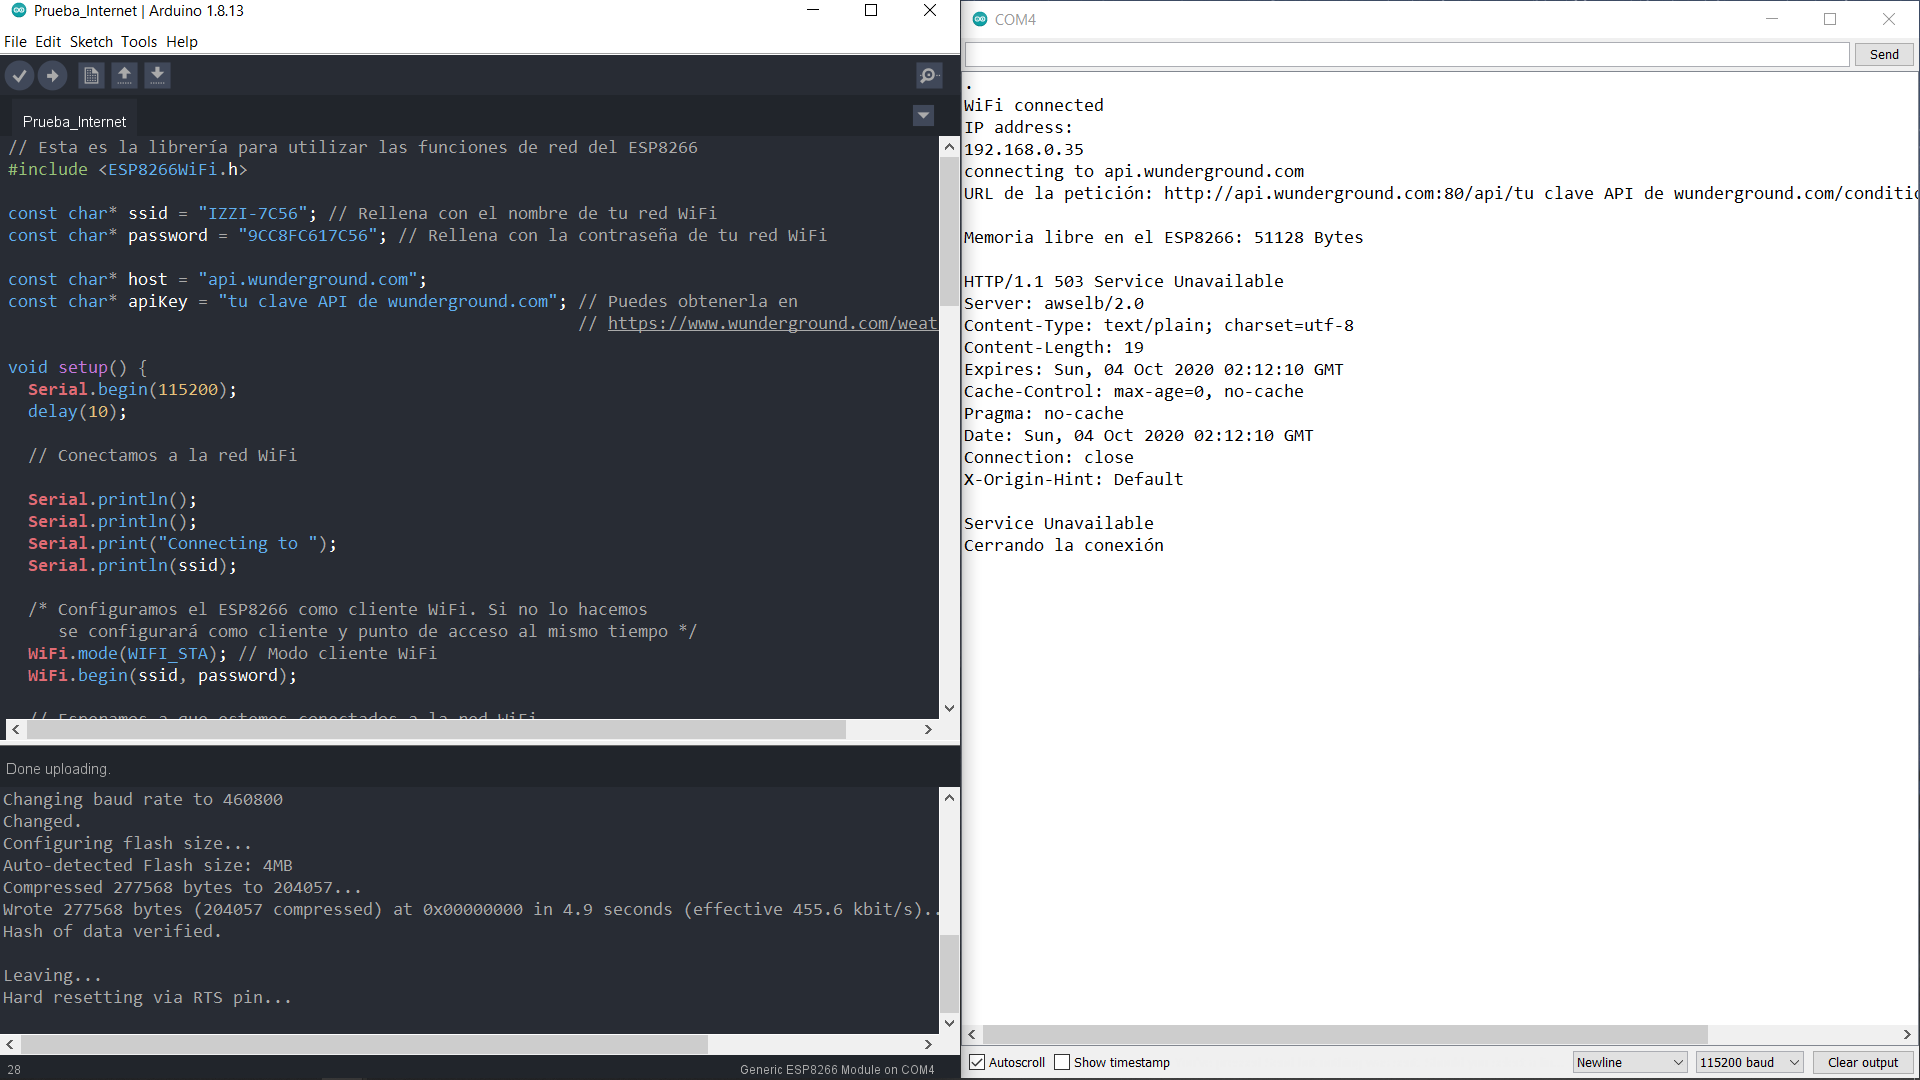
\includegraphics[width = \textwidth]{axel2}
\end{figure}

\newpage

\subsection{Jesús Urquidez Calvo}
\begin{figure}[!h]
\centering
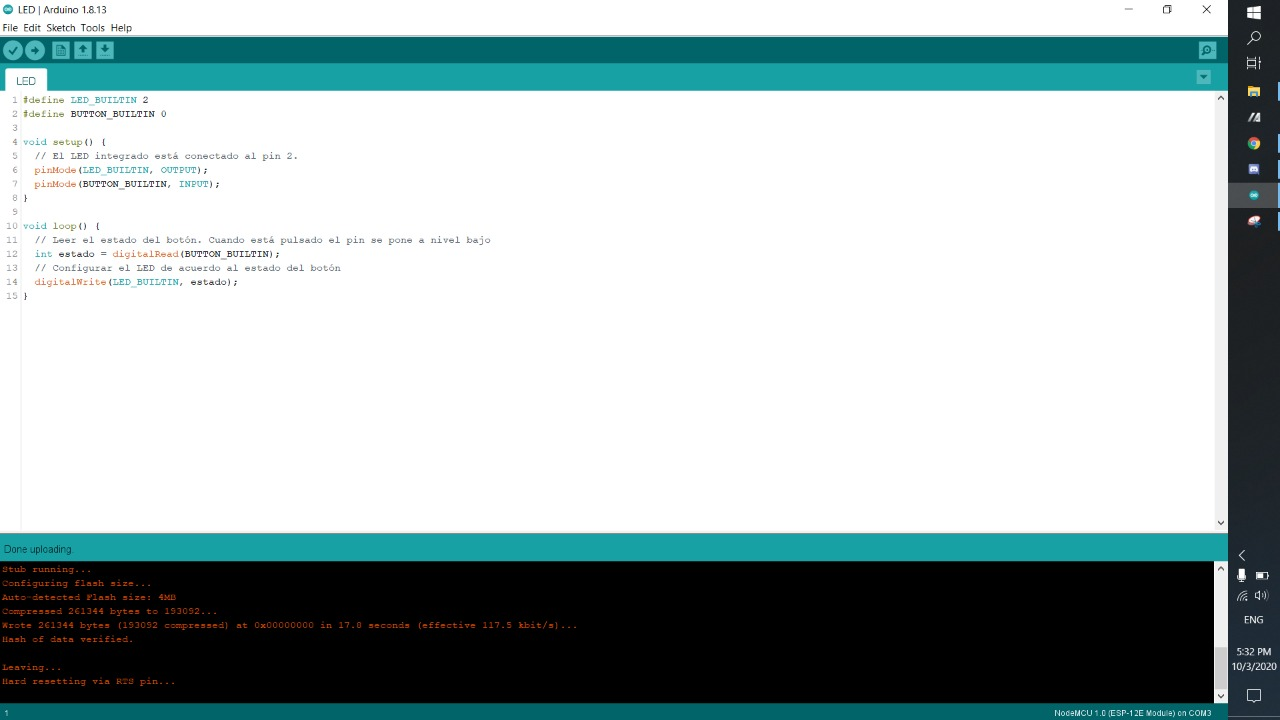
\includegraphics[width = \textwidth]{gsus1}
\end{figure}

\begin{figure}[!h]
\centering
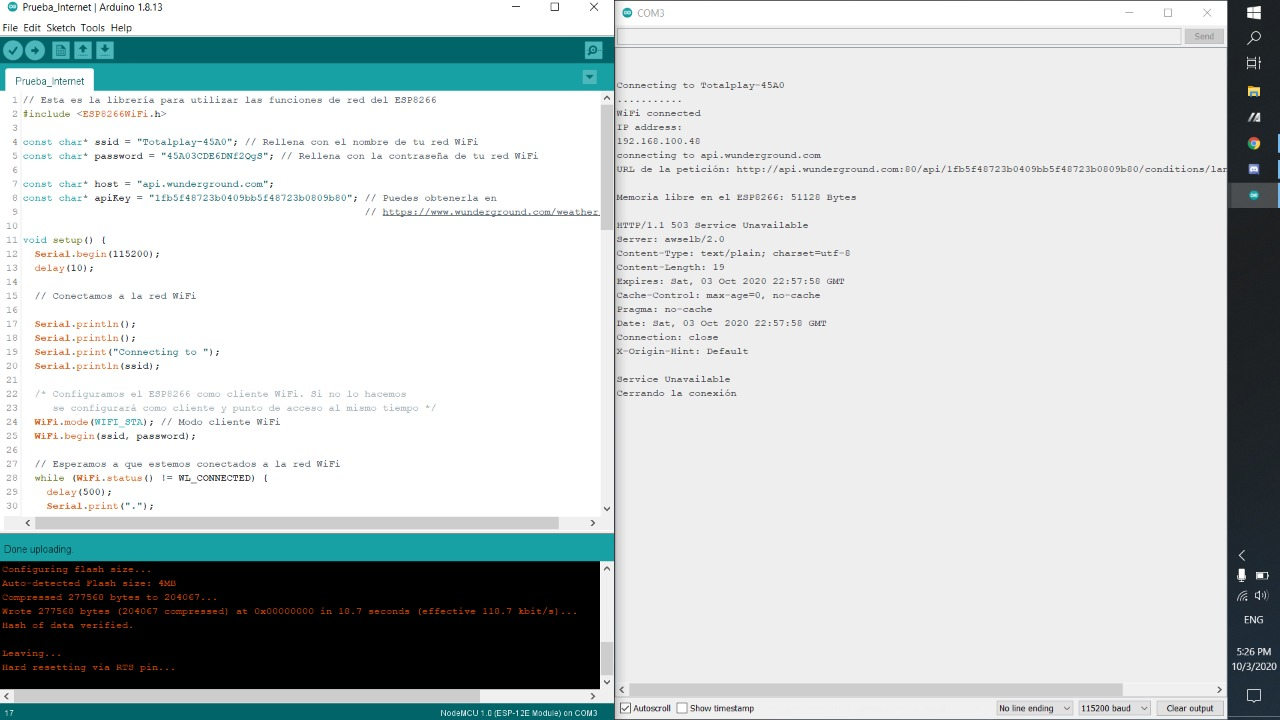
\includegraphics[width = \textwidth]{gsus2}
\end{figure}

\newpage

\subsection{Guillermo Andrés Castillo Chapa}
\begin{figure}[!h]
\centering
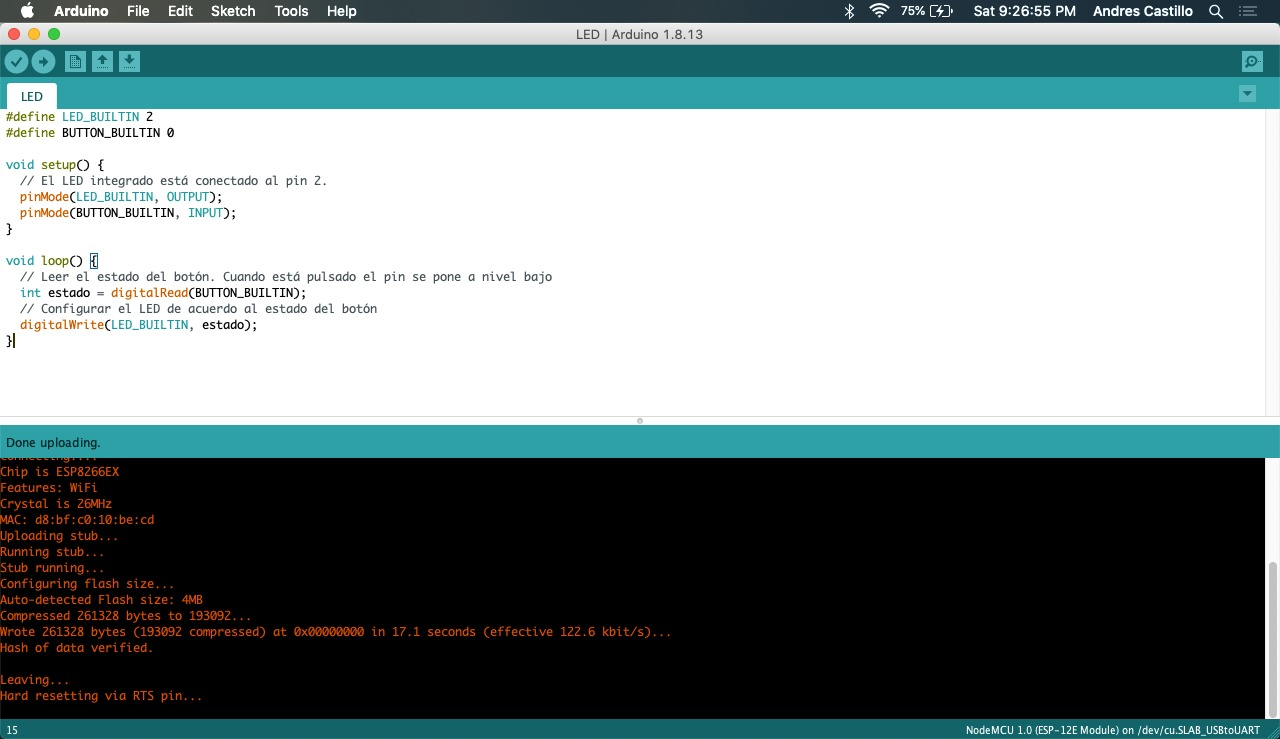
\includegraphics[width = \textwidth]{andres1}
\end{figure}

\begin{figure}[!h]
\centering
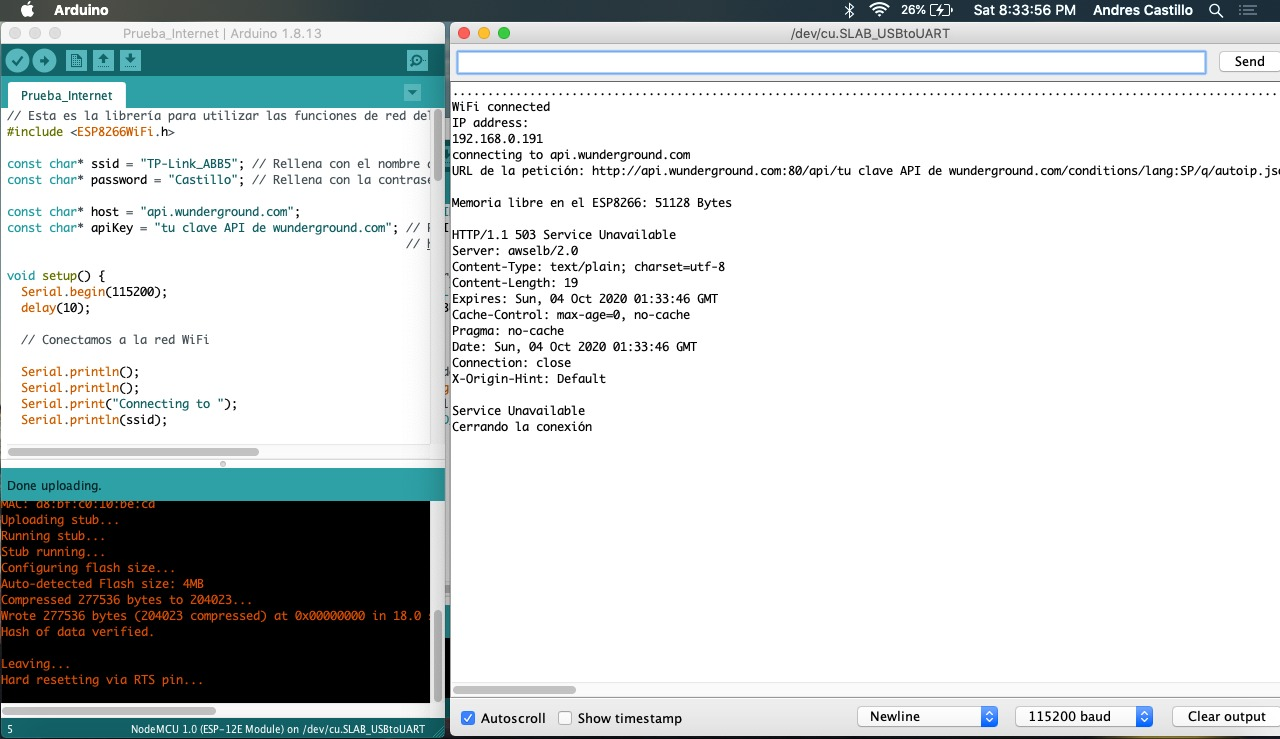
\includegraphics[width = \textwidth]{andres2}
\end{figure}

\newpage

\section{Evidencias Planeación}\label{evidencia_Planeacion}
\begin{figure}[!h]
\centering
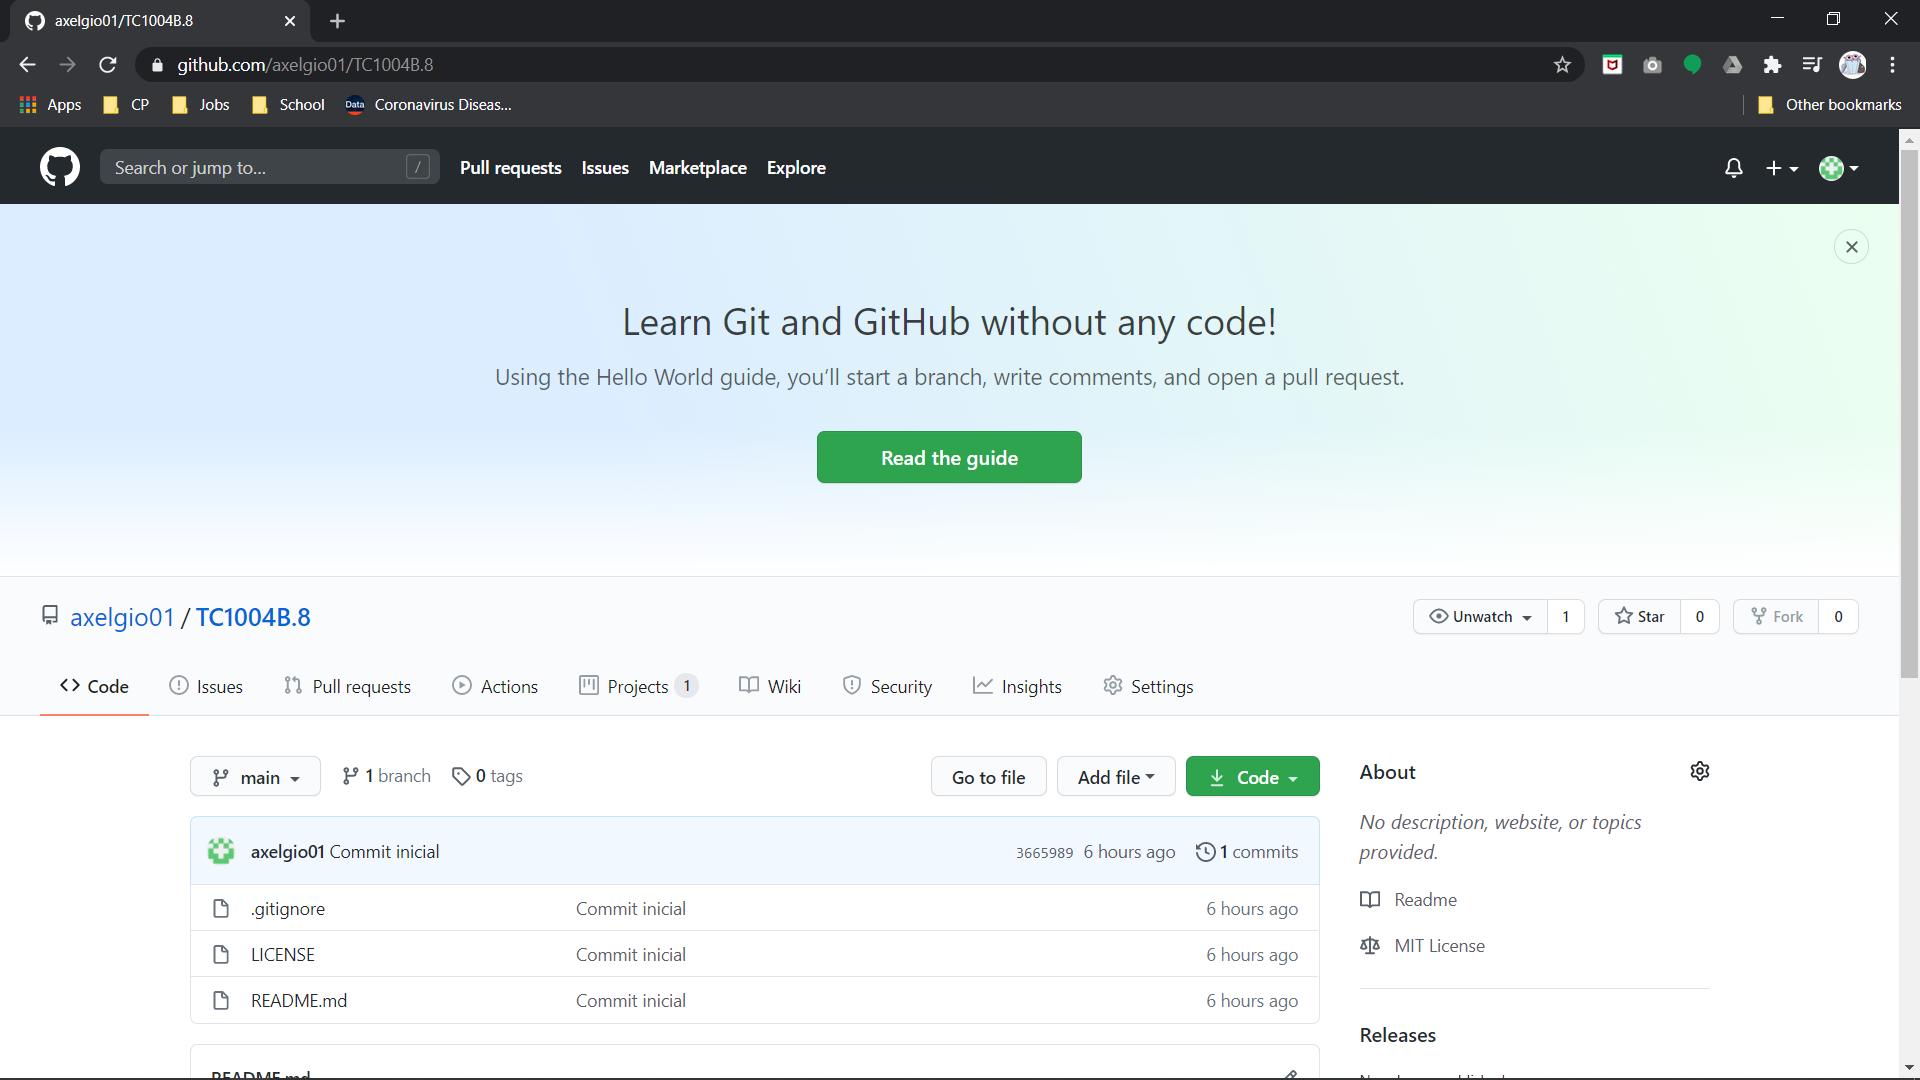
\includegraphics[width = \textwidth]{repo_Inicio}
\end{figure}

\begin{figure}[!h]
\centering
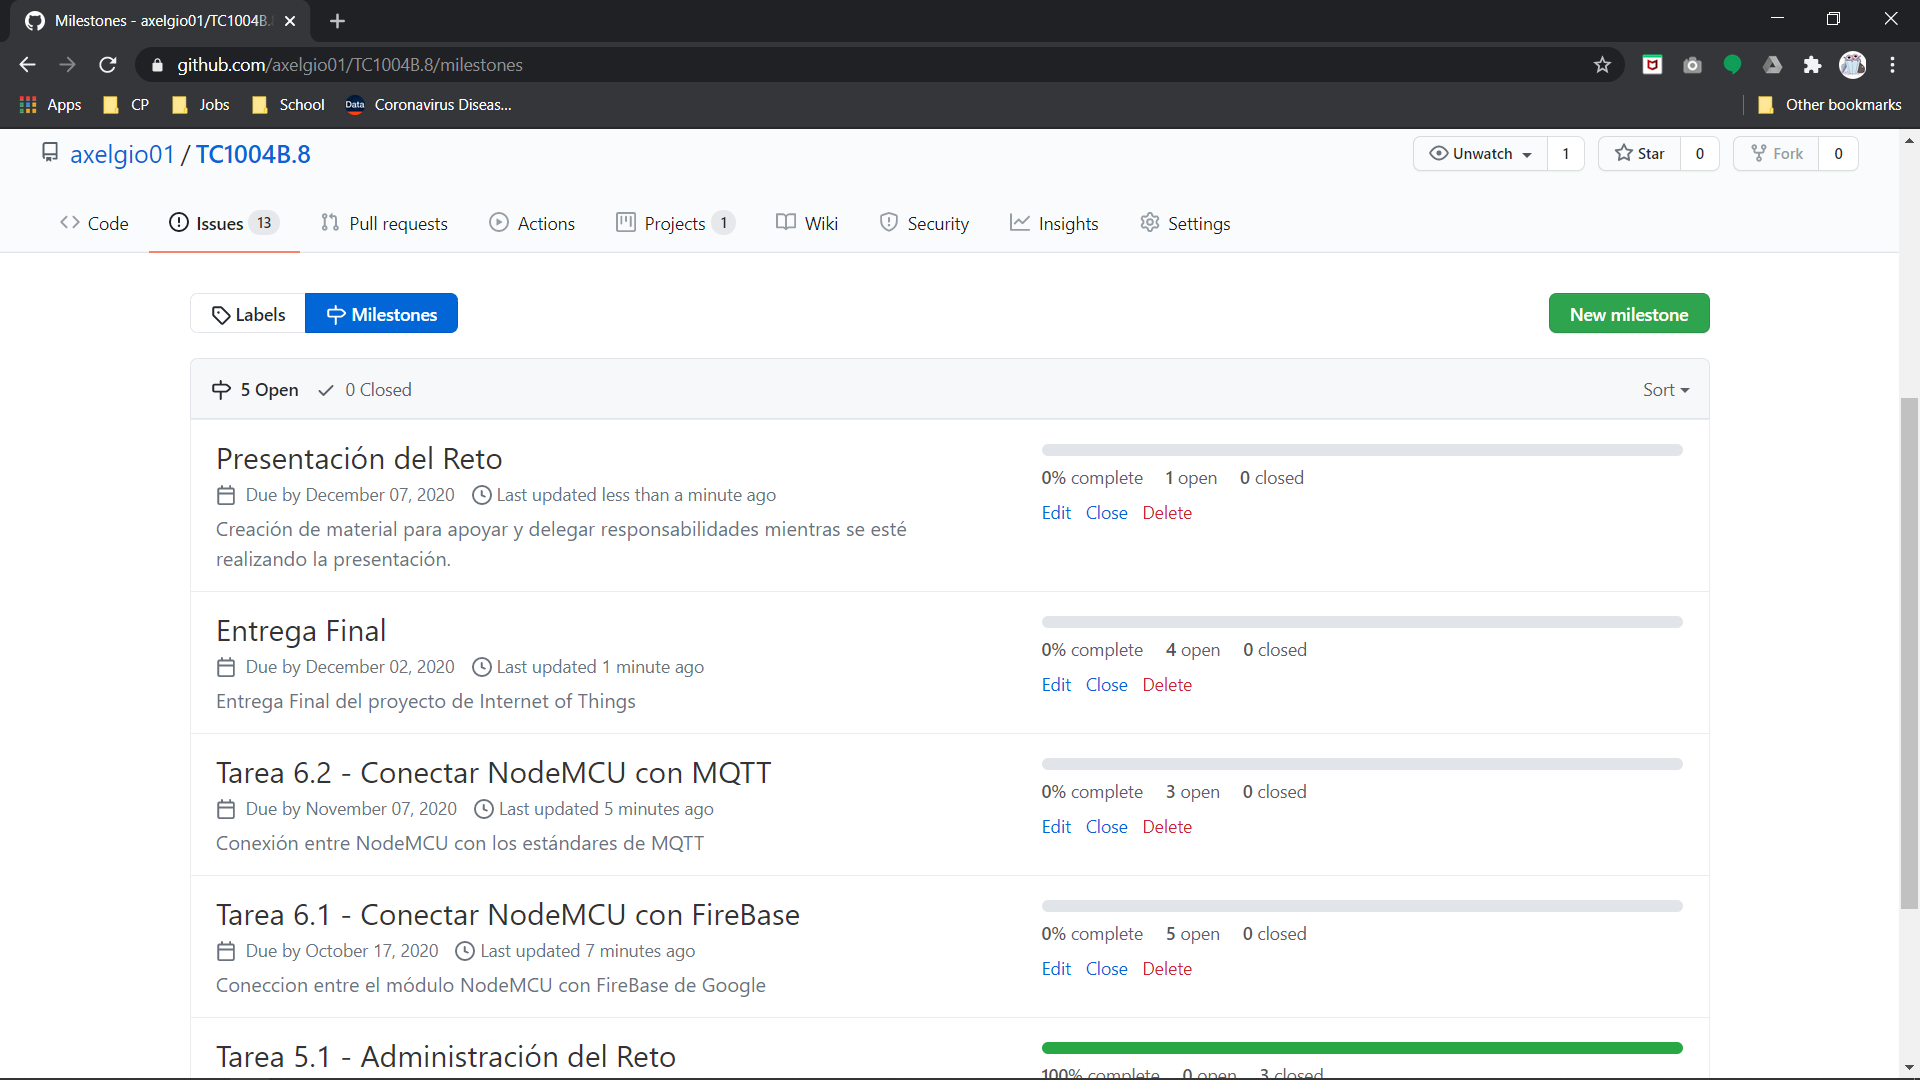
\includegraphics[width = \textwidth]{repo_Milestones}
\end{figure}

\newpage

\begin{figure}[!h]
\centering
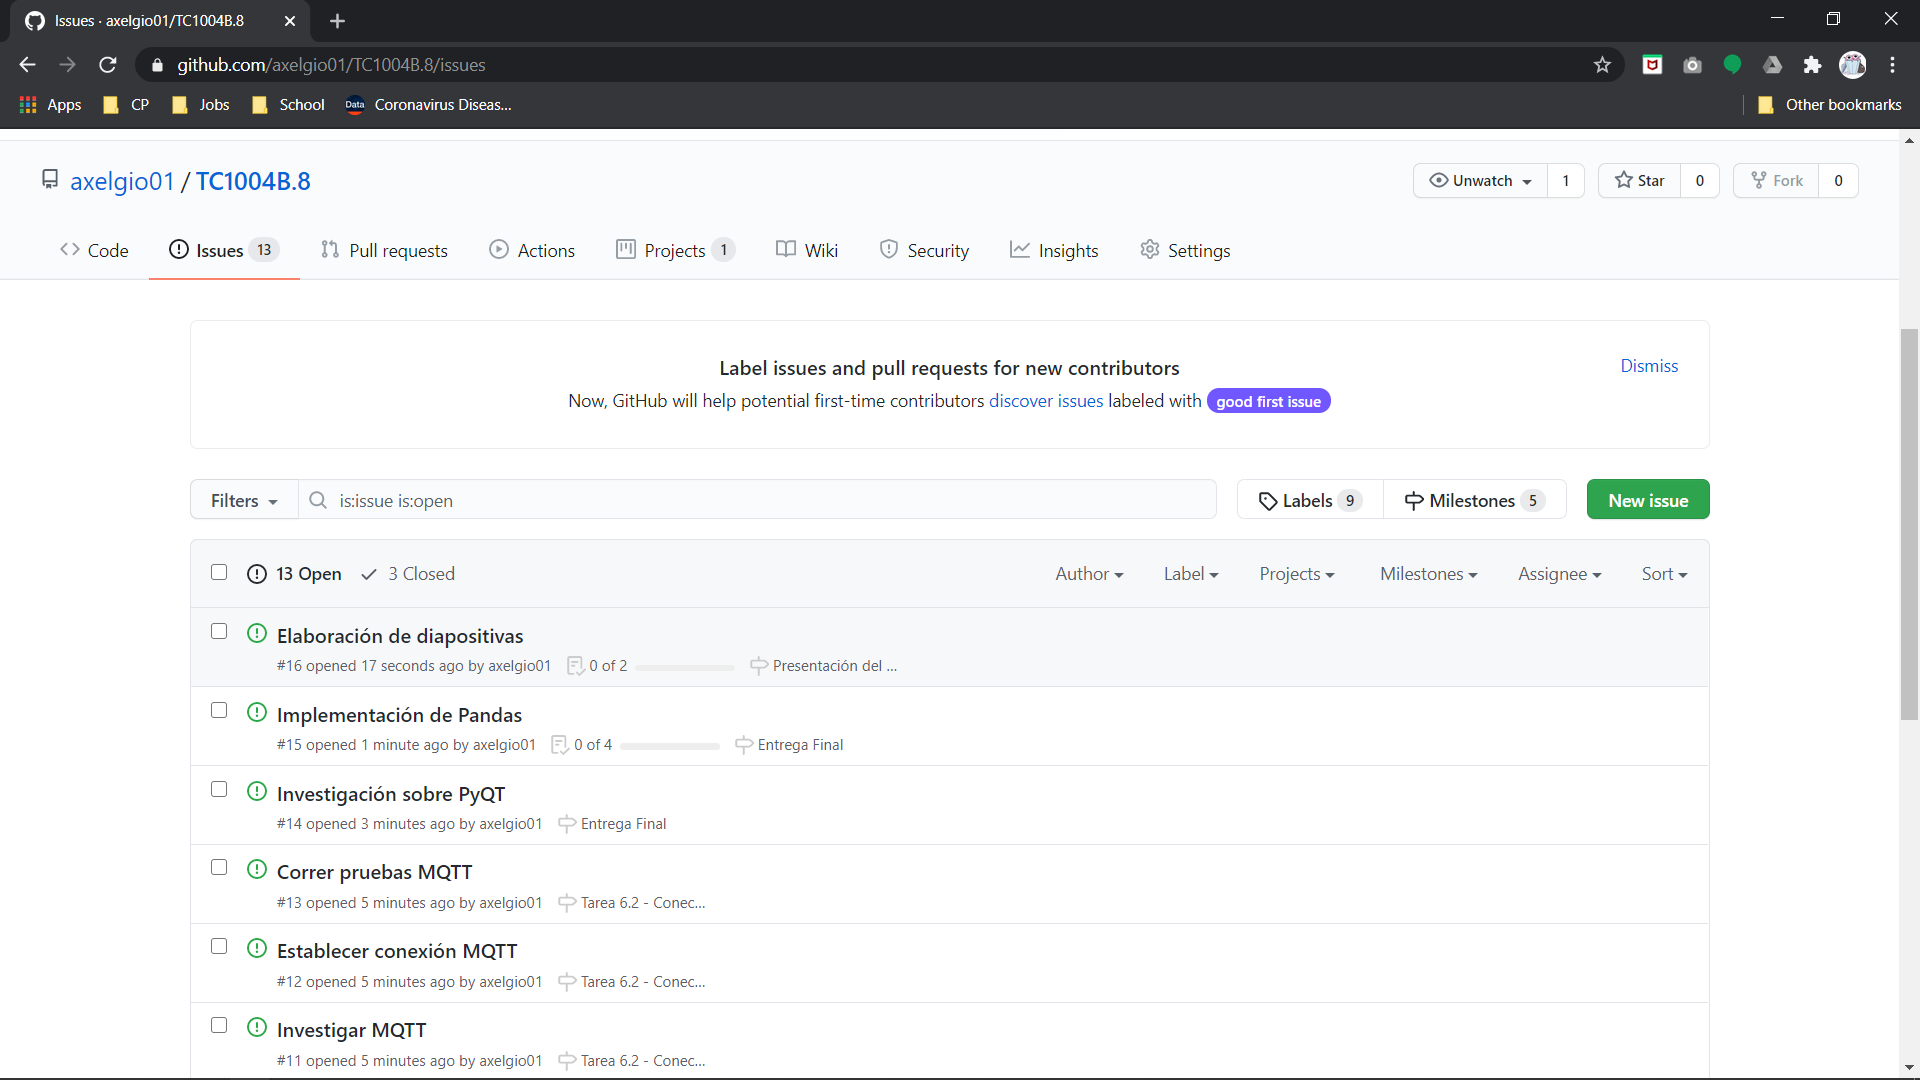
\includegraphics[width = \textwidth]{repo_Issues}
\end{figure}

\end{document}